\section{Agentic Stock Analysis Design}
\label{sec:agentic-stock-analysis-design}

The principal analytical feature of Stockrium is implemented as a stateful directed graph rather than as one monolithic language-model prompt. The graph separates planning, evidence preparation, specialist analysis, synthesis, and deterministic post-processing. This separation is important because the three evidence domains have different structures: price series require numerical calculation, financial statements require multi-year and industry-aware comparison, and articles require relevance filtering and qualitative interpretation. Treating them as independent branches also makes it possible to disable selected evidence, diagnose a weak branch, and reuse the same components in live analysis and historical evaluation.

LangGraph provides the state-graph abstraction used to declare nodes, edges, shared state, and parallel branches \cite{langgraph2026graphapi}. The language model is used where semantic interpretation or natural-language synthesis is required, while Python functions retain control over interval selection, indicator calculation, technical scoring, confidence calculation, veto conditions, and price-boundary enforcement. The resulting design is therefore hybrid: it benefits from the explanatory ability of a language model without assigning every numerical or safety-sensitive decision to generated text.

\subsection{Graph Topology and Shared State}
\label{subsec:analysis-graph-state}

The compiled analysis graph contains five nodes: an orchestrator, three specialist branches, and an aggregator. Figure~\ref{fig:analysis-graph-topology} presents the execution topology. After the orchestrator creates a plan, LangGraph activates the article, fundamental, and technical nodes from the same state. Each branch writes its own entry into the shared result dictionary. The dictionary uses a merge reducer, so branch updates are combined rather than allowing the last completed branch to replace earlier results. The aggregator is executed only after the specialist branches have reached their outgoing edges.

\begin{figure}[H]
    \centering
    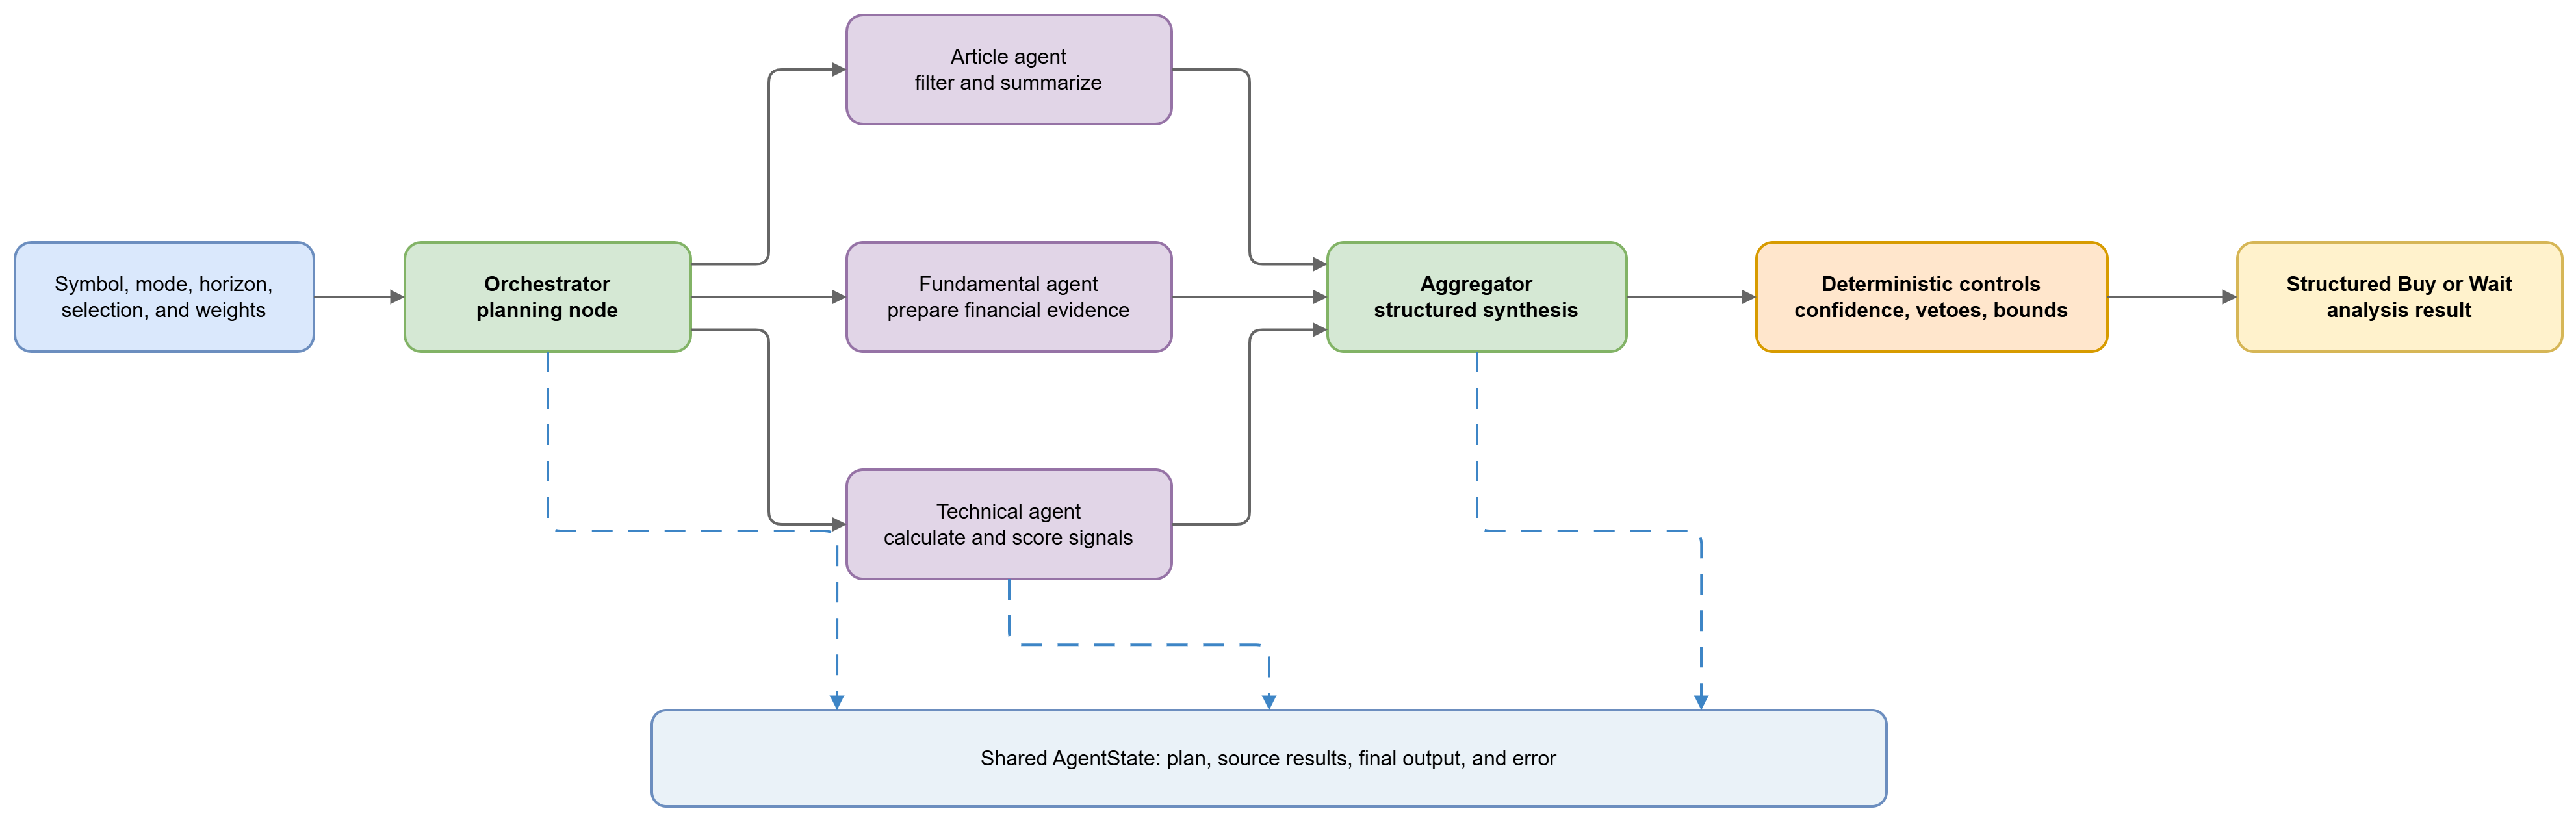
\includegraphics[width=\textwidth,keepaspectratio]{diagrams/chapter4/stockrium_agent_topology.png}
    \caption{Execution topology of the Stockrium analysis graph}
    \label{fig:analysis-graph-topology}
\end{figure}

The shared \texttt{AgentState} is a typed dictionary containing the fields summarized in Table~\ref{tab:analysis-agent-state}. State is the contract between graph nodes: a node reads only the context it requires and returns only the fields it changes. The graph can consequently add or replace a specialist without redesigning the public HTTP request.

\begin{table}[H]
    \centering
    \caption{Principal fields in the analysis graph state}
    \label{tab:analysis-agent-state}
    \small
    \setlength{\tabcolsep}{5pt}
    \renewcommand{\arraystretch}{1.18}
    \begin{tabular}{p{3.0cm} p{3.0cm} p{6.5cm}}
        \toprule
        \textbf{Field} & \textbf{Producer} & \textbf{Purpose} \\
        \midrule
        \texttt{mode} & API service & Distinguishes automatic and manual analysis; the state type also permits reuse by chat-related execution. \\
        \texttt{user\_input} & API service & Vietnamese task statement supplied to planning and final synthesis. \\
        \texttt{risk\_appetite} & API service & Contains the user's selected investment horizon, which drives time scale, default weights, and numerical bounds. \\
        \texttt{symbol} & API service & Identifies the Vietnamese listed stock being analyzed. \\
        \texttt{data\_selection} & API service & Contains enabled news, technical indicators, fundamental groups, and optional manual weights. \\
        \texttt{plan} & Orchestrator & Supplies date ranges and the deterministic technical interval to specialist nodes. \\
        \texttt{agent\_results} & Specialist nodes & Merged dictionary containing separate article, fundamental, and technical evidence. \\
        \texttt{final\_output} & Aggregator & Structured recommendation, scores, confidence, explanations, and conditional risk values. \\
        \texttt{error} & Any terminal failure & Carries a pipeline error back to the application service. \\
        \bottomrule
    \end{tabular}
\end{table}

Automatic and manual requests enter the same graph. In automatic mode, the application service replaces the submitted selection with an empty configuration; selection normalization interprets every missing switch as enabled and applies horizon-based default weights. In manual mode, the user's switches and weights remain in the state. All three graph branches are still reached structurally, but a disabled branch returns a clear disabled-source marker instead of performing unnecessary data interpretation or model work. This approach keeps the topology stable while making behavior configurable.

\subsection{Orchestration and Horizon-Aware Planning}
\label{subsec:analysis-orchestrator-planning}

The orchestrator converts the request and horizon into a structured plan. It calls \texttt{gpt-4o-mini} with temperature zero and parses the response into a Pydantic \texttt{OrchestratorPlan}. Structured output is preferable to parsing arbitrary prose because both the article and technical branches require valid \texttt{YYYY-MM-DD} boundaries \cite{openaiStructuredOutputs2026}. The prompt defines a recent lookback of approximately 60 days for short-term analysis, 180--365 days for medium-term analysis, and at least 730 days for long-term analysis. The end date is the current date.

The model does not choose the candle interval. After parsing the generated dates, Python overwrites the technical interval according to the normalized investment horizon. Short-term requests use daily candles, medium-term requests use weekly candles, and long-term requests use monthly candles. If the horizon is absent or unrecognized, the system defaults to the medium-term configuration. This deterministic mapping prevents prompt variation from assigning inconsistent analytical scales to users with the same horizon.

The fundamental branch is intentionally not given a horizon-specific number of financial years. It examines up to the five latest annual periods regardless of whether the user selected a short-, medium-, or long-term profile. This asymmetry is deliberate: the horizon changes the sensitivity of price signals, but company quality should not be inferred from a single recent accounting period. The aggregator later changes the relative influence of the fundamental evidence according to the horizon.

\subsection{Specialist Evidence Agents}
\label{subsec:analysis-specialist-agents}

The specialist nodes do not all use the language model in the same way. The technical node is primarily deterministic, the fundamental node prepares a structured textual evidence package without making the final recommendation, and the article node uses a model to filter and summarize natural-language news. Table~\ref{tab:specialist-agent-responsibilities} highlights these differences.

\begin{table}[H]
    \centering
    \caption{Responsibilities and outputs of specialist analysis nodes}
    \label{tab:specialist-agent-responsibilities}
    \small
    \setlength{\tabcolsep}{4pt}
    \renewcommand{\arraystretch}{1.2}
    \begin{tabular}{p{2.45cm} p{3.2cm} p{4.8cm} p{2.6cm}}
        \toprule
        \textbf{Node} & \textbf{Evidence} & \textbf{Processing} & \textbf{Branch output} \\
        \midrule
        Technical & Historical OHLCV candles and the most recent available price & Indicator calculation, latest-versus-previous comparison, deterministic binary scoring, and missing-value sanitation & Indicator values, explanations, current price, \texttt{total\_score}, and \texttt{max\_score} \\
        Fundamental & Annual financial indicators, statements, company profile, ICB classification, and precomputed industry medians & Five-year ordering, CAGR, DuPont preparation, sector-specific metric selection, and industry comparison & Evidence text organized by financial category \\
        Article & Stored articles related to the symbol within the planned dates & Date filtering, compact evidence construction, relevance screening, and model-based summary of benefits and risks & Vietnamese news summary or an explicit no-data marker \\
        \bottomrule
    \end{tabular}
\end{table}

\subsubsection{Technical-Analysis Agent}
\label{subsubsec:technical-analysis-agent}

The technical agent first obtains the most recent one-minute price when live analysis is being performed. It separately loads candles in the horizon-selected interval and date range. Daily records are aggregated by the market service when weekly or monthly analysis is requested. The indicator service calculates moving averages, RSI, Bollinger Bands, MACD, and KDJ. During backtesting, the same node can use a historical indicator source and suppress current-price lookup so that a future price is not introduced into a past decision.

Each enabled indicator contributes at most one point. The scoring rules are shown in Table~\ref{tab:technical-signal-scoring}. They focus on a positive transition or strengthening condition rather than assigning a point whenever an indicator has any valid value. A missing indicator receives zero and an explanatory reason. The denominator is the number of indicators enabled by the user, not a fixed value of five, which keeps the later 60\% threshold meaningful in manual mode.

\begin{table}[H]
    \centering
    \caption{Deterministic positive-signal conditions in the technical agent}
    \label{tab:technical-signal-scoring}
    \footnotesize
    \setlength{\tabcolsep}{4pt}
    \renewcommand{\arraystretch}{1.18}
    \begin{tabular}{p{1.65cm} p{10.9cm}}
        \toprule
        \textbf{Indicator} & \textbf{One-point condition; satisfying any listed condition is sufficient} \\
        \midrule
        RSI & Crosses upward through 50; is between 50 and 70 and rising; or is below 35 but recovering from the previous value. \\
        Moving averages & SMA20 crosses upward through SMA50; SMA20 remains above SMA50 with an expanding positive gap; or current price is above SMA20 while SMA20 is above SMA50. \\
        Bollinger Bands & Price crosses upward through the middle band; remains above the middle band with a widening positive distance; or recovers while at or below the lower band. \\
        MACD & MACD crosses upward through its signal line; MACD is above the signal while the histogram strengthens; or the histogram changes from negative to nonnegative. \\
        KDJ & K crosses upward through D; K is above D while J strengthens; or K rises while below 20. \\
        \bottomrule
    \end{tabular}
\end{table}

For every enabled indicator, the output contains current and previous values, a binary score, and a rule-generated reason. The agent also returns the actual covered dates, number of candles, interval, and display price. The aggregator can therefore ask the language model to explain concrete signals while retaining a score that was produced outside the model. Overbought RSI, price above the upper Bollinger Band, weakening MACD histogram, or overbought KDJ can be described as cautionary evidence even though the system's recommendation vocabulary remains limited to Buy and Wait.

\subsubsection{Fundamental-Analysis Agent}
\label{subsubsec:fundamental-analysis-agent}

The fundamental agent loads financial indicators, income statements, cash flows, a stored summary, and company-profile metadata. It retains up to five most recent annual records and orders them chronologically. For applicable values it computes compound annual growth rate as

\begin{equation}
    \operatorname{CAGR}(x) = \left(\frac{x_{n}}{x_{0}}\right)^{\frac{1}{y_{n}-y_{0}}} - 1,
    \label{eq:fundamental-cagr}
\end{equation}

where $x_{0}$ and $x_{n}$ are the earliest and latest positive observations and $y_{n}-y_{0}$ is the elapsed number of years. CAGR is omitted when fewer than two valid points exist, the elapsed period is nonpositive, or either endpoint is nonpositive. This restriction avoids producing a misleading growth percentage for a series that changes sign.

For nonfinancial firms, selected evidence is organized into liquidity, leverage, efficiency, profitability, and valuation. The leverage or profitability preparation can include a DuPont decomposition,

\begin{equation}
    ROE = \text{Net Margin} \times \text{Asset Turnover} \times \text{Financial Leverage},
    \label{eq:dupont-stockrium}
\end{equation}

which helps distinguish margin-driven returns from efficient asset use or debt-supported returns. For firms whose ICB code begins with 8, the agent uses a financial-sector presentation based on available CAMELS-related measures. It avoids relying on P/E and EV/EBITDA for financial-sector valuation and instead presents P/B. When specialized measures such as CAR, NPL, NIM, LDR, or CIR are unavailable, the evidence explicitly states the limitation rather than filling it with an inferred value.

The company is also compared with precomputed annual medians for the corresponding ICB industry. A comparison table is included only when at least three peers contribute, reducing the risk of treating one or two companies as a representative benchmark. The evidence includes the latest company value, latest industry median, company CAGR, and industry CAGR for selected measures. These deterministic preparations give the aggregator concrete relative context rather than asking it to decide what constitutes the industry from an unrestricted prompt.

Disabling every fundamental category causes the branch to return an explicit disabled marker. Data-access failures and completely missing financial records are converted to a no-data marker and do not terminate the other branches. This is important for newly listed companies and for batch analysis, where one incomplete company should not cancel an entire universe.

\subsubsection{Article-Analysis Agent}
\label{subsubsec:article-analysis-agent}

The article agent retrieves records already associated with the selected stock and filters them to the orchestrator's date interval. Its input to the model contains each article's date, title, available summary, and stored sentiment. The model is instructed to retain useful and relevant content and return a Vietnamese structure containing the main information, positive points, and negative points or risks. This branch uses a low but nonzero temperature of 0.2 because limited linguistic variation is acceptable in a summary, while highly variable creative output is undesirable in financial analysis.

If the user disables news, no article falls within the planned period, or the branch cannot provide usable content, it returns a recognizable marker. The aggregator detects these markers in Python. Missing news is therefore treated as absent evidence rather than silently converted into neutral evidence that would still affect confidence.

\subsection{Aggregation and Structured Recommendation}
\label{subsec:analysis-aggregation}

The aggregator receives the three branch results and first determines which sources contain real evidence. Technical data is active only if the result is a dictionary containing indicators and no error. Fundamental and article text are active only if they are nonempty and do not contain known disabled or no-data markers. These flags are placed into the aggregation prompt so the model cannot legitimately fill an absent section with invented analysis.

The model parses its response into an \texttt{InvestmentRecommendation} schema. The schema restricts the recommendation to \textit{Mua} (Buy) or \textit{Chờ} (Wait); requires separate technical, fundamental, news, and summary explanations; and carries the raw labels needed by deterministic confidence calculation. It also permits entry, take-profit, stop-loss, and maximum-holding values only for a candidate Buy result. A structured schema guarantees field presence and type conformance, but it does not by itself guarantee factual correctness. Stockrium therefore applies Python post-processing after parsing.

The aggregator's prompt requires technical explanations to cover each enabled indicator, fundamental explanations to use the appropriate nonfinancial or financial-sector structure, and news explanations to distinguish macro-level, company-level, and outlook implications. It also instructs the model not to repeat the recommendation or invent confidence inside narrative fields. If generation reaches the configured output-token limit, the aggregator retries once with an instruction to shorten each explanation. Any unrecovered aggregation exception places an error in graph state and produces a safe Wait-shaped fallback with empty risk values.

\subsection{Deterministic Confidence and Decision Controls}
\label{subsec:analysis-deterministic-controls}

Confidence is calculated after structured parsing and must not be interpreted as a probability of future profit. Let $s_t$ be the technical score and $m_t$ the number of enabled technical indicators. The normalized source components are

\begin{equation}
    c_t = \frac{s_t}{m_t}, \qquad
    c_f \in \{1, 0.5, 0\}, \qquad
    c_n \in \{1, 0.5, 0\},
    \label{eq:confidence-components}
\end{equation}

where fundamental labels \texttt{strong}, \texttt{neutral}, and \texttt{weak} map respectively to $1$, $0.5$, and $0$, while article labels \texttt{positive}, \texttt{neutral}, and \texttt{negative} use the same mapping. If no technical indicator is enabled, the technical component is set to $0$; in that configuration the technical source is inactive and is removed by the effective-weight renormalization in Equation~\ref{eq:effective-confidence}, so this value does not affect the final confidence.

Default weights vary by horizon as shown in Table~\ref{tab:confidence-horizon-weights}. The short-term profile emphasizes price signals, while the long-term profile emphasizes company fundamentals. Manual weights replace this table after API validation has established that the three values are within $[0,1]$ and total one.

\begin{table}[H]
    \centering
    \caption{Default confidence weights by investment horizon}
    \label{tab:confidence-horizon-weights}
    \small
    \renewcommand{\arraystretch}{1.2}
    \begin{tabular}{lccc}
        \toprule
        \textbf{Horizon} & \textbf{Technical} & \textbf{Fundamental} & \textbf{News} \\
        \midrule
        Short term: below 3 months & 0.60 & 0.10 & 0.30 \\
        Medium term: 3--12 months & 0.40 & 0.40 & 0.20 \\
        Long term: above 1 year & 0.15 & 0.70 & 0.15 \\
        \bottomrule
    \end{tabular}
\end{table}

An unavailable or disabled source is removed before aggregation. If $A$ is the set of active sources and $w_i$ is the default or manual base weight, the effective weight is

\begin{equation}
    w_i^{\prime} =
    \begin{cases}
        \displaystyle\frac{w_i}{\sum_{j \in A} w_j}, & i \in A,\\[6pt]
        0, & i \notin A,
    \end{cases}
    \qquad
    C = \sum_i w_i^{\prime}c_i.
    \label{eq:effective-confidence}
\end{equation}

Thus, disabling news does not leave its original weight as an invisible neutral contribution. The remaining evidence is renormalized to sum to one. The response exposes the component scores, effective weights, raw technical score, qualitative labels, final confidence, and the fixed acceptance threshold of $0.55$, making the calculation inspectable.

The decision layer acts conservatively as a veto system. The model is first instructed to apply the same rules and generates a candidate recommendation. Python never promotes a model-generated Wait to Buy; it can only preserve a candidate Buy or downgrade it. A candidate Buy is changed to Wait when any applicable condition holds:

\begin{itemize}
    \item the technical score is below $\lceil 0.60m_t \rceil$, provided at least one technical indicator is enabled;
    \item fundamental evidence exists and its label is \texttt{weak};
    \item news evidence exists and its label is \texttt{negative}; or
    \item deterministic confidence is below $0.55$.
\end{itemize}

If fundamental or news evidence is absent, its veto is skipped rather than treated as a negative signal. If the final result is Wait, all trading-plan values are set to \texttt{null}. This long-only design prevents the result from resembling a short-sale or execution instruction and is consistent with the application scope.

For a surviving Buy result, the current technical price is used when the model does not supply an entry price. Python then constrains take-profit distance, stop-loss distance, and maximum holding count according to Table~\ref{tab:horizon-price-boundaries}. An out-of-range value is clamped to the nearest boundary; a missing or invalid value is replaced by the midpoint of the permitted range. Final prices are recalculated from the bounded percentages and appended to the narrative summary only after enforcement, preventing the displayed text from disagreeing with the structured numerical fields.

\begin{table}[H]
    \centering
    \caption{Implemented horizon-specific trading-plan boundaries}
    \label{tab:horizon-price-boundaries}
    \small
    \setlength{\tabcolsep}{7pt}
    \renewcommand{\arraystretch}{1.2}
    \begin{tabular}{lccc}
        \toprule
        \textbf{Horizon} & \textbf{Take-profit distance} & \textbf{Stop-loss distance} & \textbf{Maximum hold} \\
        \midrule
        Short term & 8--15\% above entry & 4--7\% below entry & 5--15 candles \\
        Medium term & 15--30\% above entry & 7--12\% below entry & 15--60 candles \\
        Long term & 40--80\% above entry & 15--20\% below entry & 120--260 candles \\
        \bottomrule
    \end{tabular}
\end{table}

Two implementation qualifications are necessary for an accurate description. First, the prompt asks the model to maintain a reward-to-risk ratio of at least 1.5, but the current Python post-processing does not recalculate this condition as a final veto after clamping. The ratio displayed in the result is therefore informative rather than a deterministically guaranteed constraint. Second, the boundary configuration describes maximum hold in daily-candle terms, while live technical analysis maps medium- and long-term horizons to weekly and monthly candles and the mobile interface labels the field as a number of candles. The present code does not convert the bounded count between these time scales. Consequently, the values in Table~\ref{tab:horizon-price-boundaries} document the implementation but should not be reinterpreted as a universally consistent calendar duration. Aligning interval semantics and adding a final reward-to-risk assertion are appropriate hardening tasks for future work.

Overall, the agentic workflow separates evidence acquisition and deterministic calculation from semantic synthesis. Parallel specialist nodes make each analytical perspective inspectable; structured models constrain generated objects; and Python checks can reject a candidate Buy that violates measurable rules. The workflow remains an analytical support mechanism rather than an autonomous trading system: it supplies a traceable Buy-or-Wait assessment, but it neither places an order nor guarantees an investment outcome.
